\documentclass[12pt, twoside]{article}
\usepackage[letterpaper, margin=1in]{geometry}
\usepackage[english]{babel}
\usepackage[utf8]{inputenc}
\usepackage{amsmath}
\usepackage{amsfonts}
\usepackage{amssymb}
\usepackage{tikz}
%\usetikzlibrary{quotes, angles}

\usepackage{graphicx}
\usepackage{enumitem}
\usepackage{multicol}

\usepackage{fancyhdr}
\pagestyle{fancy}
\fancyhf{}
\renewcommand{\headrulewidth}{0pt} % disable the underline of the header

\fancyhead[RE]{\thepage}
\fancyhead[RO]{\thepage \\ Name: \hspace{3cm}}
\fancyhead[L]{BECA / Dr. Huson / 10th Grade Geometry\\* 29 May 2019}

\begin{document}
\subsubsection*{13-1 Classwork: Similar triangles, dilation ratios}
 \begin{enumerate}

   \item Given $\triangle ABP$ and $\triangle JKP$ as shown below. $\overline{AB} \parallel \overline{JK}$. Prove $\triangle ABP \sim \triangle JKP$.\\[0.5cm]
     \begin{tikzpicture}[scale=1.4]
         \draw [thick]
           (0.25,-1)node[right]{$B$}--
           (-0.5,2)node[left]{$K$}--
           (4,0)node[right]{$J$}--
           (0,0)node[above right]{$P$}--
           (-2,0)node[left]{$A$}--cycle;
       \end{tikzpicture}

     \begin{multicols}{2}
       \underline{Statement} \\
       \underline{Reason}
     \end{multicols}
     \begin{multicols}{2}
       \raggedcolumns
       \begin{enumerate}[label={\arabic*)}]
         \item $\triangle ABP$, $\triangle JKP$ \vspace{0.3cm}
         \item \rule{4cm}{0.15mm} \vspace{0.3cm}
         \item $\angle APB \cong \angle JPK$  \vspace{0.3cm}
         \item $\angle PAB \cong \angle PJK$ \vspace{0.3cm}
         \item $\triangle ABP \sim \triangle JKP$ \vspace{0.3cm}
       \end{enumerate}
       \begin{enumerate}[label={\arabic*)}]
         \item Given \vspace{0.3cm}
         \item Given \vspace{0.3cm}
         \item \rule{4cm}{0.15mm} \vspace{0.3cm}
         \item \rule{4cm}{0.15mm} \vspace{0.3cm}
         \item \rule{4cm}{0.15mm} \vspace{0.3cm}
       \end{enumerate}
     \end{multicols}

     \item Triangle $ABC$ is dilated with a factor of $\frac{3}{2}$ centered at $A$, yielding $\triangle ADE$, as shown. Given $AB=10$, $BC=12$, and $AC=14$. \\[0.25cm] Find $AD$, $AE$, and $DE$. \vspace{1cm}
     \begin{center}
         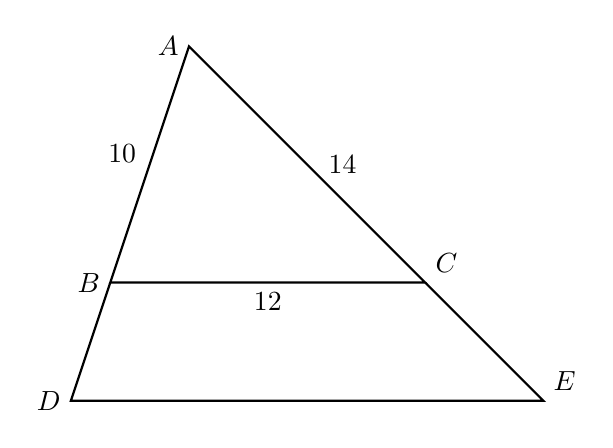
\begin{tikzpicture}[scale=0.5]
           \draw [thick]
           (0,0)node[left]{$B$}--
           (8,0)node[above right]{$C$}--
           (2,6)node[left]{$A$}--cycle;
           \draw [thick]
           (0,0)--
           (-1,-3)node[left]{$D$}--
           (11,-3)node[above right]{$E$}--(8,0);
           \node at (4,0)[below]{$12$};
           \node at (5.3, 3)[right]{$14$};
           \node at (0.3, 2.8)[above]{$10$};
         \end{tikzpicture}
       \end{center}

  \newpage

  \item Triangle $ADE$ is drawn with $\overline{BC} \parallel \overline{DE}$, as shown. Given $AB=5$, $BC=7$, $AC=8$, and $BD=5$. \\[0.25cm] Find $CE$, $AE$, and $DE$.
  \begin{center}
      \begin{tikzpicture}[scale=0.65]
        \draw [thick]
        (0.5,1.5)node[left]{$B$}--
        (6.5,1.5)node[above right]{$C$}--
        (2,6)node[above]{$A$}--cycle;
        \draw [thick]
        (0.5,1.5)--
        (-1,-3)node[left]{$D$}--
        (11,-3)node[above right]{$E$}--(6.5,1.5);
        \node at (3,1.5)[below]{$7$};
        \node at (4.5, 4)[right]{$8$};
        \node at (0.6, 3.3)[above]{$5$};
        \node at (-0.7, -1)[above]{$5$};
      \end{tikzpicture}
    \end{center} \vspace{2cm}

  \item Given $\triangle ABP$ and $\triangle JKP$ as shown below. $\overline{AB} \parallel \overline{JK}$. $AP=5.7$, $JP=11.4$, and $JK=14.8$. Find $AB$.\\[0.5cm]
    \begin{tikzpicture}[scale=1.4]
        \draw [thick]
          (0.25,-1)node[right]{$B$}--
          (-0.5,2)node[left]{$K$}--
          (4,0)node[right]{$J$}--
          (0,0)node[above right]{$P$}--
          (-2,0)node[left]{$A$}--cycle;
      \end{tikzpicture}

\end{enumerate}
\newpage
\setcounter{page}{1}
\subsubsection*{13-1 Homework: Similar triangles, dilation ratios}
  \begin{enumerate}

    \begin{multicols}{2}
    [\item A dilation maps triangle $PQR$ onto triangle $STU$ with $QR=4$ and $TU=6$.] \vspace{0.75cm}
      \begin{enumerate}
        \item $\overline{QR} \rightarrow$ \rule{2cm}{0.15mm}
        \item Complete the fraction numerators with the corresponding segment and length: \\[0.75cm]
        $\displaystyle k=\frac{\qquad}{QR} =\frac{\qquad}{4}$
        \item What scale factor maps\\
         $\triangle PQR \rightarrow \triangle STU$?
      \end{enumerate}
      \begin{tikzpicture}[scale=0.9]
        \coordinate [label=above left:$P$](A) at (85:2);
        \coordinate [label=below:$Q$](B) at (0, 0);
        \coordinate [label=right:$R$](C) at (-20:3);
        \draw [thick] (A)--(B)--(C)--cycle;

        \draw [thick, xshift=2cm, yshift=2.5cm] (85:3) node[above]{$S$}--
        (0,0) node[below]{$T$}--
        (-20:4.5) node[right]{$U$}--cycle;
      \end{tikzpicture}
    \end{multicols}  \vspace{1cm}

  \item Triangle $ADE$ and its midline $\overline{BC}$ are drawn, with $B$ the midpoint of $\overline{AD}$ and $C$ the midpoint of $\overline{AE}$. The two medians $\overline{AE}$ and $\overline{AE}$ are drawn, as shown, intersecting in point $F$, the centroid.\\[0.25cm]
  $\triangle FCB \sim \triangle FDE$ with scale factor $k=2$.\\[0.25cm]
  Given $BC=7$, find $DE$. \\[0.25cm] Given $BF=4$, find $FE$. \vspace{1cm}
  \begin{center}
      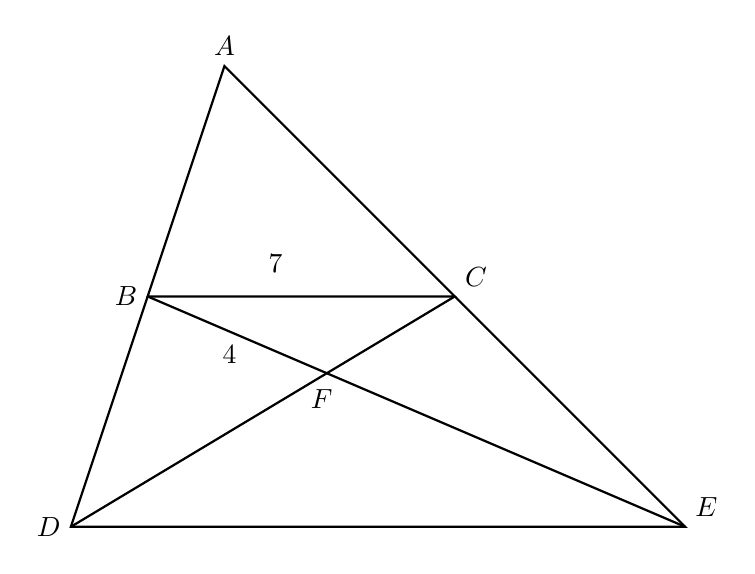
\begin{tikzpicture}[scale=0.65]
        \draw [thick]
        (0.5,1.5)node[left]{$B$}--
        (6.5,1.5)node[above right]{$C$}--
        (2,6)node[above]{$A$}--cycle;
        \draw [thick]
        (0.5,1.5)--
        (-1,-3)node[left]{$D$}--
        (11,-3)node[above right]{$E$}--(6.5,1.5);
        \draw [thick] (0.5,1.5)--(11,-3);
        \draw [thick] (6.5,1.5)--(-1,-3);
        \node at (3,2.5)[below]{$7$};
        \node at (3.5, -0.5)[right]{$F$};
        \node at (2.1, 0)[above]{$4$};
        %\node at (-0.7, -1)[above]{$5$};
      \end{tikzpicture}
    \end{center}


\end{enumerate}
\end{document}
